\documentclass{beamer}
% Replace the \documentclass declaration above
% with the following two lines to typeset your 
% lecture notes as a handout:
% \documentclass{article}
% \usepackage{beamerarticle}
\usepackage{hyperref}
\usepackage{graphicx}
\usepackage{tikz}
\usetikzlibrary{arrows.meta}
\usetikzlibrary{decorations.pathreplacing,angles,quotes}
\usepackage{subcaption}
\usepackage{amsmath}
\usepackage{amssymb}
\usepackage{multirow}
\usetheme[progressbar=frametitle]{metropolis}
\usepackage{pgfplots}
\pgfplotsset{width=\textwidth,compat=1.9}

% \usepackage{fontspec}
% \setmainfont[
%   Ligatures=TeX,
%   BoldFont=OpenDyslexicAlta-Bold.otf,
%   ItalicFont=OpenDyslexicAlta-Italic.otf,
%   BoldItalicFont=OpenDyslexicAlta-BoldItalic.otf
% ]{OpenDyslexic-Regular.otf}

\usetheme[progressbar=frametitle]{metropolis}


\usepackage{pgfplots}
\pgfplotsset{width=\textwidth,compat=1.9}

\usepackage{graphicx}
\usepackage{tikz}
\usetikzlibrary{arrows.meta}
\usetikzlibrary{decorations.pathreplacing,angles,quotes}
\usepackage{subcaption}
\usepackage{amsmath}
\usepackage{amssymb}
\usepackage{multirow}

\newcommand{\R}{\mathbb{R}}
\newcommand{\doublebar}[2][0]{\skew#1\bar{\textit{\b #2}}}

\usepackage{booktabs}
\usepackage[scale=2]{ccicons}

\usepackage{pgfplots}
\usepgfplotslibrary{dateplot}

\usepackage{xspace}
\definecolor{UniBlue}{RGB}{0, 48, 135}
\definecolor{UniRed}{RGB}{203, 51, 59}

\definecolor{cbOrange}{RGB}{230,159,0}
\definecolor{cbSkyBlue}{RGB}{86,180,233}
\definecolor{cbBluishGreen}{RGB}{0,158,115}
\definecolor{cbYellow}{RGB}{240, 228, 66}
\definecolor{cbBlue}{RGB}{0, 114, 178}
\definecolor{cbVermillion}{RGB}{213, 94, 0}
\definecolor{cbReddishPurple}{RGB}{204, 121, 167}

\setbeamercolor{title}{fg=UniBlue}
\setbeamercolor{frametitle}{bg=white,fg=UniBlue}
\setbeamercolor{structure}{fg=UniRed}
\setbeamercolor{alerted text}{fg=UniBlue}

\newcommand{\themename}{\textbf{\textsc{metropolis}}\xspace}

\title{Primer on Grain Markets
}
\subtitle{AGBU 230}
% \date{\today}
\date{Winter 2017-2018}
\author{Jason Holderieath, PhD}
\institute{Louisiana Tech University \\ School of Agricultural Sciences and Forestry \\
Developed from Price Analysis: A Fundamental Approach to the Study of Commodity Prices by Mindy L. Mallory 2017-11-30}
\titlegraphic{\hfill
\includegraphics[height=1.5cm]{AGR_sch_sci_for_logo.pdf}}

\begin{document}
%\metroset{titleformat frame=allsmallcaps}
\maketitle


\begin{frame}[<+-| alert@+>]{Grain and Oilseed Markets}
\begin{itemize}
\item Chapter contains basic biological and time-lines.
\item major grains and oilseeds: 
\begin{itemize}
\item Corn
\item Soybeans
\item Hard Red Winter Wheat (KC wheat)
\item Hard Red Spring Wheat (Minneapolis wheat)
\item Soft Red Winter Wheat
\end{itemize}
\end{itemize}
%Notes: 

\end{frame}

\section{Corn}

\begin{frame}[<+-| alert@+>]{Sweet and Field Corn}
What's the difference between Sweet Corn one buys from the grocery store and field corn (the focus of much of this course)?

\begin{itemize}
\item Sweet Corn
\begin{itemize}
\item Bred so that the kernels contain a high sugar content.
\item Harvested green.
\item Must be consumed or processed quickly.
\end{itemize}
\item Field Corn
\begin{itemize}
\item Corn belt corn is planted from about March to May
\item Pollination occurs in July
\item Harvested from September to October
\item Since pollination is key to production and yield, new crop futures prices tend to be highly variable in the months of June and July. 
\item Weather during planting and harvest is also of interest to markets.
\end{itemize}
\end{itemize}
\end{frame}



\begin{frame}[<+-| alert@+>]{Recent Trends in Acreage, Yields, Production, and Use}
\begin{itemize}
\item Recently around 90 million acres each year.
\item Corn and soybeans said to be 'competing for acres' based on new crop prices.
\item Hybrids and genetics.

\end{itemize}

\end{frame}

\begin{frame}{2016 Corn Planted Acres}
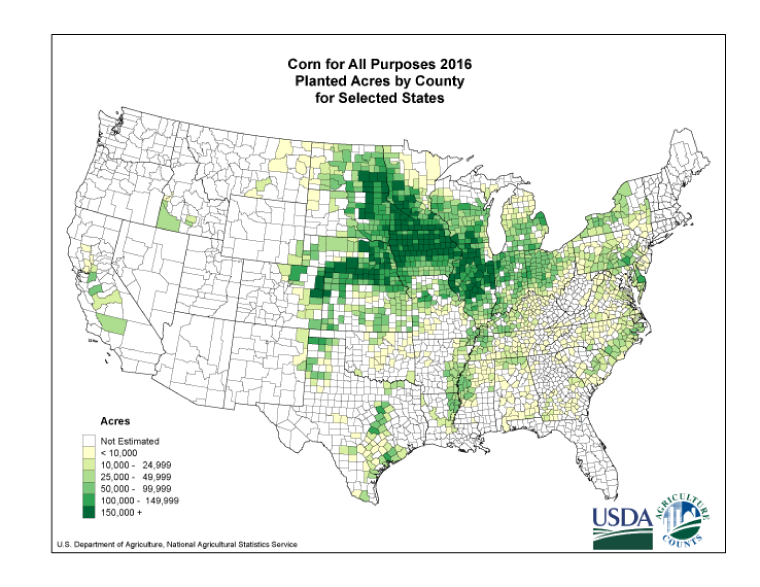
\includegraphics[width=\textwidth]{Corn-PA-2016.png}
\end{frame}

\begin{frame}{Corn Planted Acres and Yield}
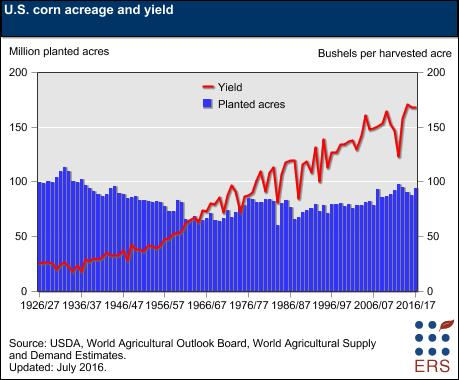
\includegraphics[width=.75\textwidth]{Corn-PA-Yield.png}
\end{frame}

\begin{frame}{Corn Price Received by Farmers and Production}
Corn prices can be quite volatile, with prices and production highly inversely related to one another
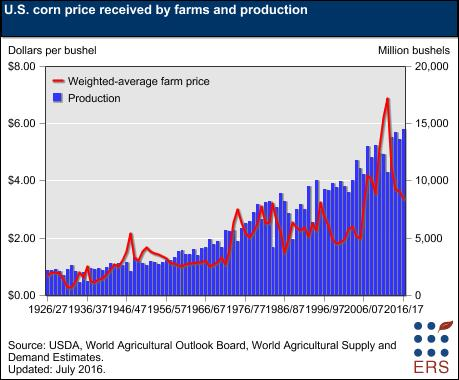
\includegraphics[width=.75\textwidth]{Corn-PriceR-Production.png}
\end{frame}

\begin{frame}{Corn Domestic Use Categories}
Corn is used in the U.S for a variety of purposes. Largest use categories are feed (for livestock), and alcohol for fuel use (ethanol blended with gasoline).
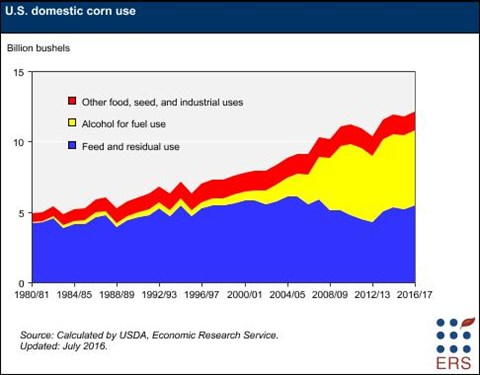
\includegraphics[width=.75\textwidth]{Corn-Domestic-Use.png}
\end{frame}

\begin{frame}{Largest Exporters of Corn}
Corn is a global commodity, and the U.S. is the worlds largest producer and exporter of corn. 
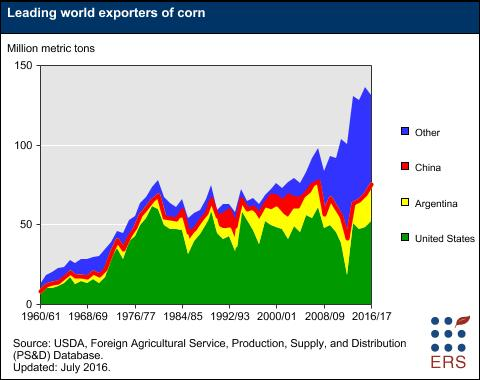
\includegraphics[width=.75\textwidth]{Corn-World-Exporters.png}
\end{frame}

\begin{frame}{Largest Importers of Corn}
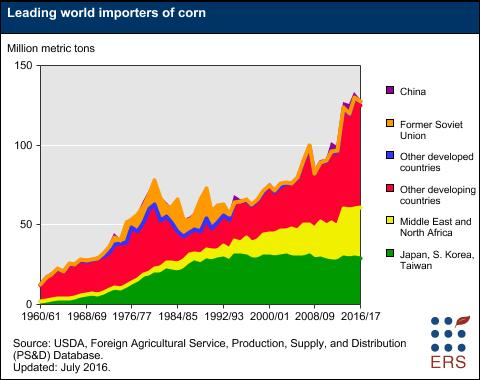
\includegraphics[width=.75\textwidth]{Corn-World-Importers.png}
\end{frame}

\section{Soybeans}

\begin{frame}[<+-| alert@+>]{Soybeans}
\begin{itemize}
\item Soybeans are planted later than corn (approx. April to June)
\item Weather affects soybean production prospects.
\item Soybean prices, therefore are highly dependent on what happens during the summer months.
\item Soybeans did not begin to be commercially grown in the U.S. until the mid 20th century.
\item Biotechnology
\end{itemize}
\end{frame}

\begin{frame}{Soybean Planted Acres and Yield}
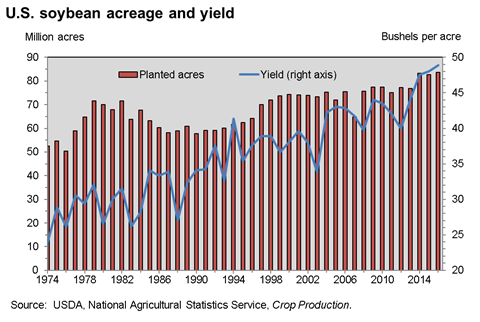
\includegraphics[width=.8\textwidth]{Soy-Acres-Yield.png}
\end{frame}

\begin{frame}{Domestic Soybean Use}
\begin{itemize}
\item Soybeans consumed in the U.S. are almost exclusively processed into soybean meal and soybean oil, a process referred to as 'crushing'. 
\item Soybean meal is high in protein and used as an ingredient in livestock feed.
\item Soybean oil is used for a variety of things, but the bulk of it is consumed as edible oil.
\end{itemize}
\end{frame}

\begin{frame}{U.S. Soybean Exports}
About half of the soybeans produced in the U.S. are exported, and more than half of soybeans exported are imported by China.
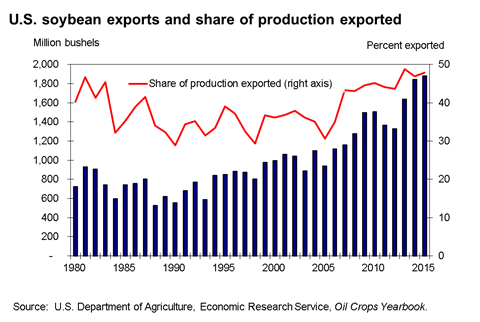
\includegraphics[width=.75\textwidth]{Soy-Exports-Share-Production.png}
\end{frame}

\section{Wheat}

\begin{frame}[<+-| alert@+>]{Wheat}
\begin{itemize}
\item Three Main Types grown in the U.S.
\begin{itemize}
\item Hard Red Winter Wheat (HRW/KC Wheat)
\item Hard Red Spring Wheat (HRS/Minneapolis wheat)
\item Soft Red Winter Wheat (SRW/Chicago Wheat)
\end{itemize}
\item Each of these types of wheat have its own futures contract
\item Are grown in distinct regions of the country
\item Have different end uses
\item Primary difference is protein is contained in the kernels
\end{itemize}
\end{frame}

\begin{frame}{Wheat Variety Growing Areas}
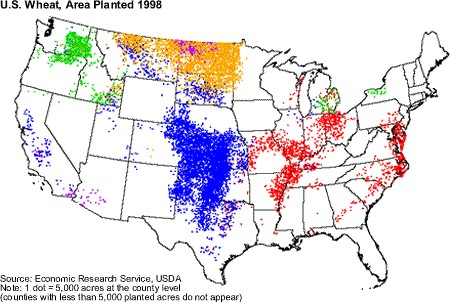
\includegraphics[width=.75\textwidth]{Wheat-Growing-Areas.jpg}

Blue = HRW, Gold = HRS, Red  = SRW
\end{frame}

\subsection{Hard Red Winter Wheat}

\begin{frame}[<+-| alert@+>]{HRW Wheat}
\begin{itemize}
\item Planted in the fall and lays dormant or grows very little during the winter.
\item Looks like grass before it is mature.
\item During April and May the wheat plants make 'heads.'
\item When the plants die the grain is harvested.
\item Primarily used to make bread flour.
\item Sometimes called Kansas City Wheat
\end{itemize}
\end{frame}
  
\begin{frame}{Hard Red Winter Wheat}
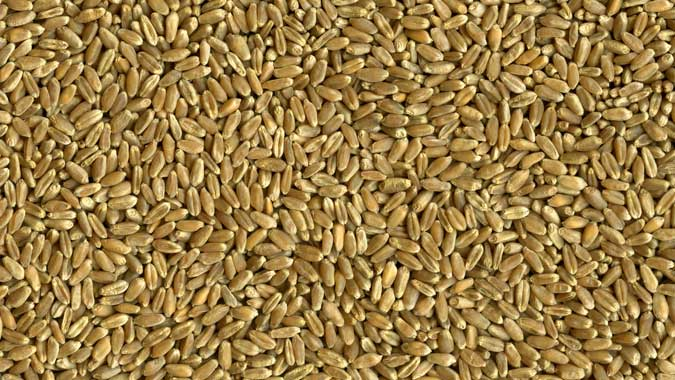
\includegraphics[width=.75\textwidth]{HRW-Wheat.jpg}
\end{frame}

\subsection{Hard Red Spring Wheat}

\begin{frame}{HRS Wheat}
\begin{itemize}
\item Planted in the spring, around April or May
\item Harvested in the fall, around September
\item Highest protein content (13-16\%)
\item High in gluten, good for baking bread.
\item Also used in wheat blends to increase protein content.
\item HRS wheat is referred to as Minneapolis Wheat
\end{itemize}
\end{frame}

\begin{frame}{Hard Red Spring Wheat}
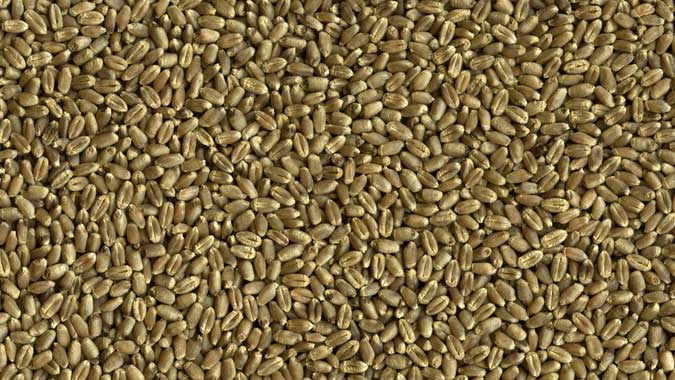
\includegraphics[width=.75\textwidth]{HRS-Wheat.jpg}
\end{frame}

\subsection{Soft Red Winter Wheat}

\begin{frame}{SRW Wheat}
\begin{itemize}
\item planted in the fall, and is harvested in the late spring
\item Lower in protein which makes is suitable for use in cakes, cookies, and crackers
\item Referred to as Chicago Wheat
\end{itemize}
\end{frame}

\begin{frame}{Soft Red Winter Wheat}
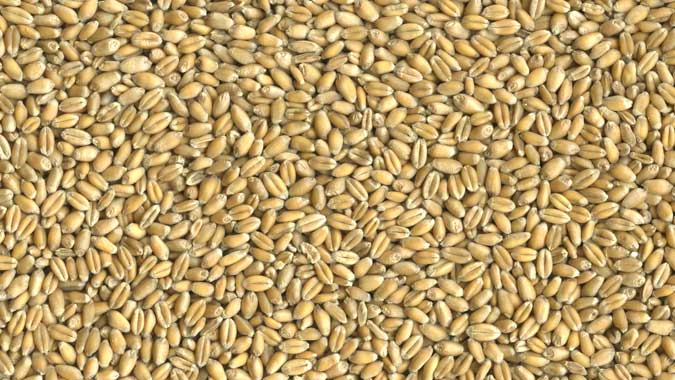
\includegraphics[width=.75\textwidth]{SRW-Wheat.jpg}
\end{frame}

\subsection{Protein Premiums and Wheat Spreads}

\begin{frame}[<+-| alert@+>]{Protein Premiums and Wheat Spreads}
\begin{itemize}
\item 'Protein premiums'
\item Flour millers rarely use just one kind of wheat
\item Different varieties of wheat naturally have different protein levels
\item Link between yield and protein levels
\begin{itemize}
\item yields are high, wheat protein is lower
\item during years where lower protein winter wheat has good yields, there is plenty of wheat, but not necessarily enough protein (So SRW prices rise against winter wheat)
\item If winter wheat crops are smaller, spring wheat may not enjoy a large premium 
\end{itemize}
\item Relative prices of Minneapolis, Kansas City, and Chicago wheat futures are closely
\end{itemize}
\end{frame}

\end{document}
